\documentclass[12pt,letterpaper]{article}

%Packages
\usepackage{pdflscape}
\usepackage{fixltx2e}
\usepackage{textcomp}
\usepackage{fullpage}
\usepackage{float}
\usepackage{latexsym}
\usepackage{url}
\usepackage{epsfig}
\usepackage{graphicx}
\usepackage{amssymb}
\usepackage{amsmath}
\usepackage{bm}
\usepackage{array}
\usepackage[version=3]{mhchem}
\usepackage{ifthen}
\usepackage{caption}
\usepackage{hyperref}
\usepackage{amsthm}
\usepackage{amstext}
\usepackage{enumerate}
\usepackage[osf]{mathpazo}
\usepackage{dcolumn}
\usepackage{lineno}
\usepackage{longtable}
\pagenumbering{arabic}

%Pagination style and stuff
\linespread{2}
\raggedright
\setlength{\parindent}{0.5in}
\setcounter{secnumdepth}{0} 
\renewcommand{\section}[1]{%
\bigskip
\begin{center}
\begin{Large}
\normalfont\scshape #1
\medskip
\end{Large}
\end{center}}
\renewcommand{\subsection}[1]{%
\bigskip
\begin{center}
\begin{large}
\normalfont\itshape #1
\end{large}
\end{center}}
\renewcommand{\subsubsection}[1]{%
\vspace{2ex}
\noindent
\textit{#1.}---}
\renewcommand{\tableofcontents}{}

\renewcommand\thefigure{C.\arabic{figure}}
\renewcommand\thetable{C.\arabic{table}}

\begin{document}

\section{Appendix C: Additional Results}

The following section contains the supplemental results of the effects of our missing data parameters and the different tree inference methods on the the ability to recover the "best" topology that are briefly discussed in the main body of the paper. For clarity, in the paper, we focused on the results of the effects of our missing data parameters on the Maximum Likelihood trees topology and the Bayesian consensus trees topology. The following additional results presented here give a greater insight into the effect of our missing data parameters on the Maximum Likelihood Bootstrapped trees topologies and the Bayesian posterior trees distribution topologies. Also we present here the pairwise comparisons between each parameters states for the Maximum Likelihood tree topology, the Maximum Likelihood Bootstrapped trees topologies and the Bayesian posterior trees distribution topologies.

\begin{figure} 
\centering
    \includegraphics[width=1\textwidth]{SupplementaryFigures/Boot+Bayt-AllParam-RF+Tr-BW.pdf}
    \caption{Effect of increasing missing data on topological recovery using Maximum Likelihood Bootstrap trees (black) and Bayesian posterior tree distribution (grey). The x axis shows the percentage of missing data from 0\% (white) to 75\% (black) for the two parameters: $M_{L}$ (upper line), $M_{F}$ (middle line) and number of characters from 100 to 25 for the parameter $N_{C}$ (lower line). Topological recovery was measured using two different tree comparison metrics: Normalised Robinson-Foulds metric (upper row) and Normalised Triplets metric (lower row). The graph shows the modal value (points), and the 50\% (thick solid lines) and 95\% (thin dashed lines) confidence intervals of the distributions of the tree comparison metric for each missing data parameter and tree inference method.} 
\label{Fig_Supp_BootBayt_allparam} 
\end{figure}

\begin{figure} 
\centering
     %Hide this figure for 'fast' build
%    \includegraphics[width=1\textwidth]{Figures/Supplementary/PairwiseComp-ML-RF+Tr-colour.pdf}
    \includegraphics[width=1\textwidth]{SupplementaryFigures/PairwiseComp-ML-RF+Tr-colour.png} %bitmap version - 300 dpi RGB
    \caption{The effects of missing data on topological recovery using Maximum Likelihood trees. The x and the y axes both show show the percentage of missing data from 0\% (white) to 75\% (black) for the two parameters: $M_{L}$ (upper line), $M_{F}$ (middle line) and number of characters from 100 to 25 for the parameter $N_{C}$ (lower line). Topological recovery is represented by the probability of (A) Normalised Robinson-Foulds metric and (B) Normalised Triplets metric distributions overlapping with the "best" tree distribution, calculated using the Bhattacharyya Coefficient. The Bhattacharyya Coefficient values are indicated using a color gradient ranging from low probability of overlap in blue, to a high probability of overlap in orange.}
\label{Fig_Supp_paircomp_ML}
\end{figure} 

\begin{figure} 
\centering
     %Hide this figure for 'fast' build
%    \includegraphics[width=1\textwidth]{Figures/Supplementary/PairwiseComp-Boot-RF+Tr-colour.pdf}
    \includegraphics[width=1\textwidth]{SupplementaryFigures/PairwiseComp-Boot-RF+Tr-colour.png} %bitmap version - 300 dpi RGB
    \caption{The effects of missing data on topological recovery using Maximum Likelihood bootstrap trees. The x and the y axes both show show the percentage ofmissing data from 0\% (white) to 75\% (black) for the two parameters: $M_{L}$ (upper line), $M_{F}$ (middle line) and number of characters from 100 to 25 for the parameter $N_{C}$ (lower line). Topological recovery is represented by the probability of (A) Normalised Robinson-Foulds metric and (B) Normalised Triplets metric distributions overlapping with the "best" tree distribution, calculated using the Bhattacharyya Coefficient. The Bhattacharyya Coefficient values are indicated using a color gradient ranging from low probability of overlap in blue, to a high probability of overlap in orange.}
\label{Fig_Supp_paircomp_Boot}
\end{figure} 

\begin{figure} 
\centering
     %Hide this figure for 'fast' build
%    \includegraphics[width=1\textwidth]{Figures/Supplementary/PPairwiseComp-Bayt-RF+Tr-colour.pdf}
    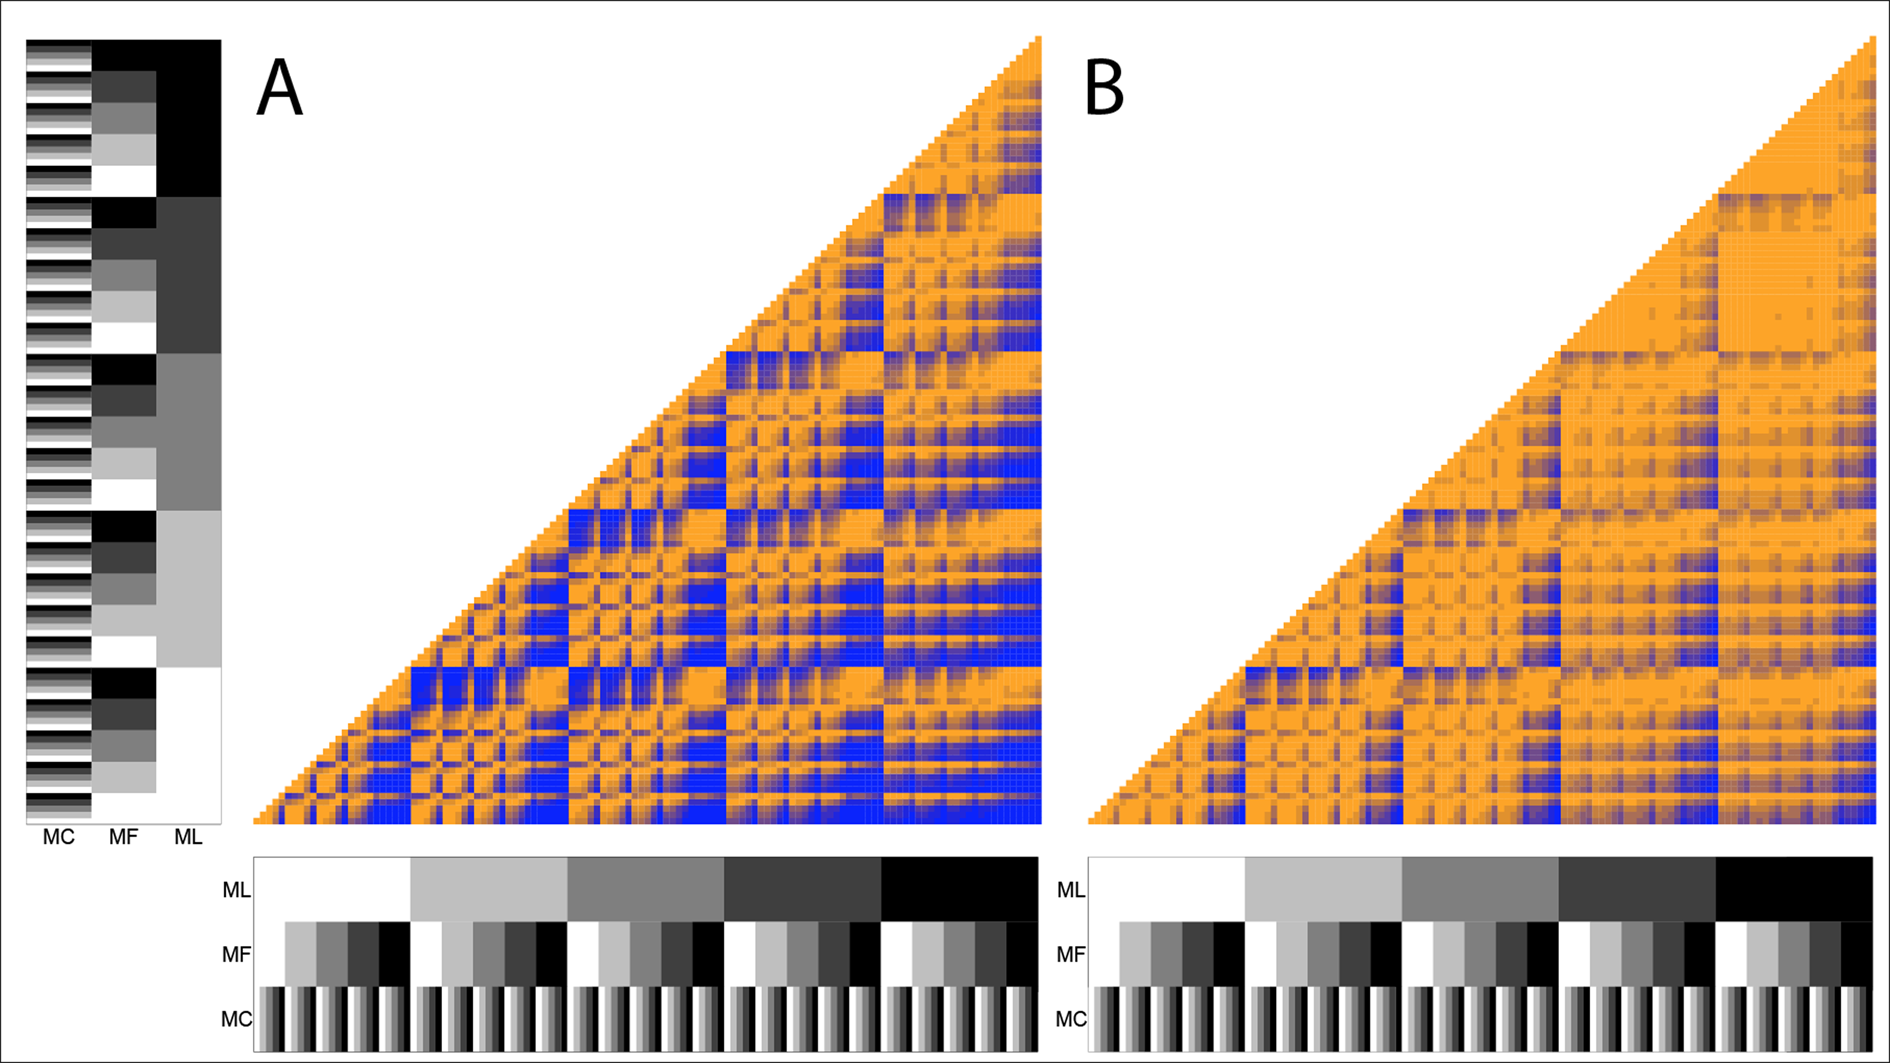
\includegraphics[width=1\textwidth]{SupplementaryFigures/PairwiseComp-Bayt-RF+Tr-colour.png} %bitmap version - 300 dpi RGB
    \caption{The effects of missing data on topological recovery using Bayesian posterior tree distribution. The x and the y axes both show show the percentage of missing data from 0\% (white) to 75\% (black) for the two parameters: $M_{L}$ (upper line), $M_{F}$ (middle line) and number of characters from 100 to 25 for the parameter $N_{C}$ (lower line). Topological recovery is represented by the probability of (A) Normalised Robinson-Foulds metric and (B) Normalised Triplets metric distributions overlapping with the "best" tree distribution, calculated using the Bhattacharyya Coefficient. TThe Bhattacharyya Coefficient values are indicated using a color gradient ranging from low probability of overlap in blue, to a high probability of overlap in orange.}
\label{Fig_Supp_paircomp_Bayt}
\end{figure} 


\begin{figure} 
\centering
    \includegraphics[width=1\textwidth]{SupplementaryFigures/Boot+Bayt-AllParam-RF+Tr-BW.pdf}
    \caption{Effect of increasing missing data on topological recovery using Maximum Likelihood Bootstrap trees (black) and Bayesian posterior tree distribution (grey). The x axis shows the percentage of missing data from 0\% (white) to 75\% (black) for the two parameters: $M_{L}$ (upper line), $M_{F}$ (middle line) and number of characters from 100 to 25 for the parameter $N_{C}$ (lower line). Topological recovery was measured using two different tree comparison metrics: Normalised Robinson-Foulds metric (upper row) and Normalised Triplets metric (lower row). The graph shows the modal value (points), and the 50\% (thick solid lines) and 95\% (thin dashed lines) confidence intervals of the distributions of the tree comparison metric for each missing data parameter and tree inference method.} 
\label{Fig_Supp_BootBayt_allparam} 
\end{figure}


\begin{figure} 
\centering
    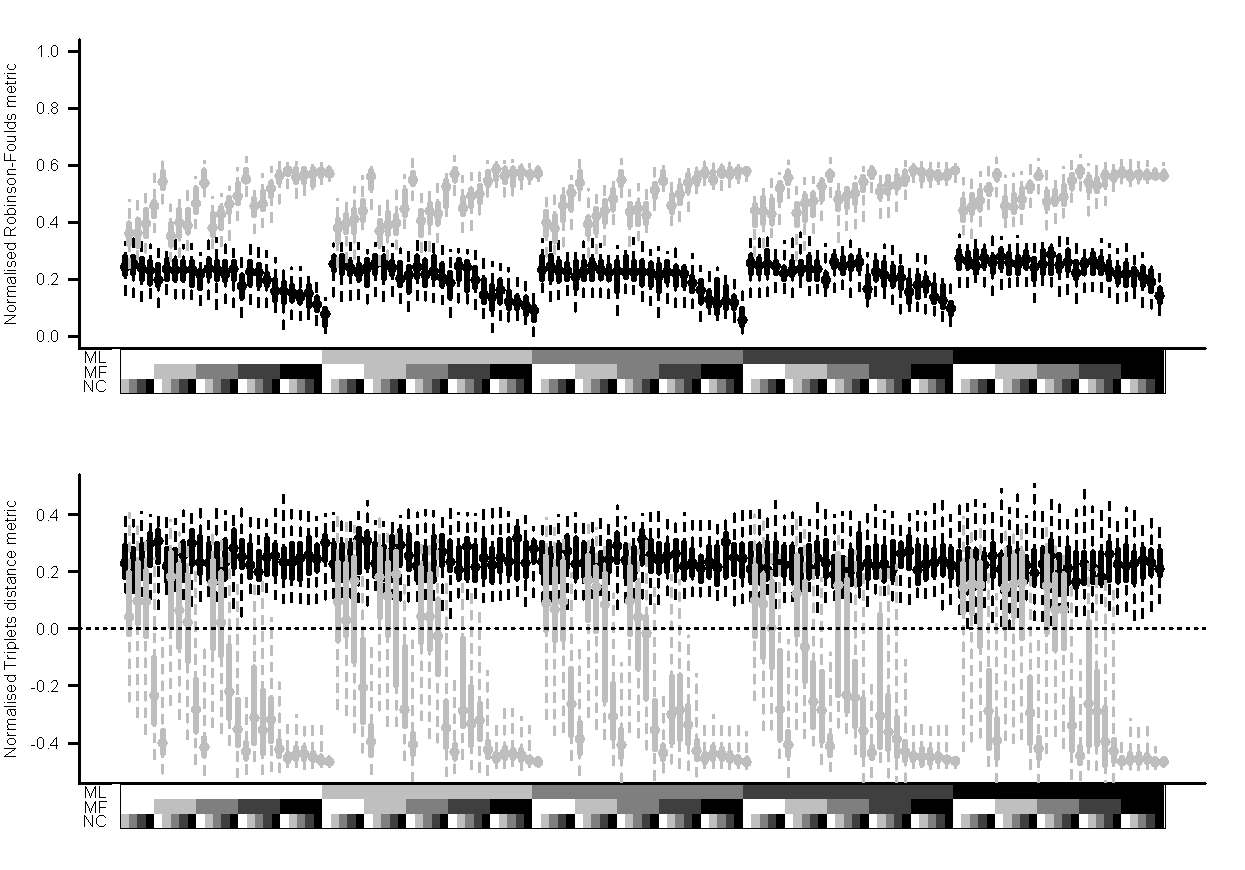
\includegraphics[width=1\textwidth]{SupplementaryFigures/Singles_True.pdf}
    \caption{Effect of increasing missing data on recovering the ``true'' tree topology (the tree used for starting our simulations) for the Maximum Likelihood trees (black) and Bayesian consensus trees (grey). The x axis shows the percentage of missing data from 0\% (white) to 75\% (black) for the two parameters: $M_{L}$ (upper line), $M_{F}$ (middle line) and number of characters from 100 to 25 for the parameter $N_{C}$ (lower line). Topological recovery was measured using two different tree comparison metrics: Normalised Robinson-Foulds metric (upper row) and Normalised Triplets metric (lower row). The graph shows the modal value (points), and the 50\% (thick solid lines) and 95\% (thin dashed lines) confidence intervals of the distributions of the tree comparison metric for each missing data parameter and tree inference method.} 
\label{Fig_Supp_Singles_true} 
\end{figure}


\begin{figure} 
\centering
    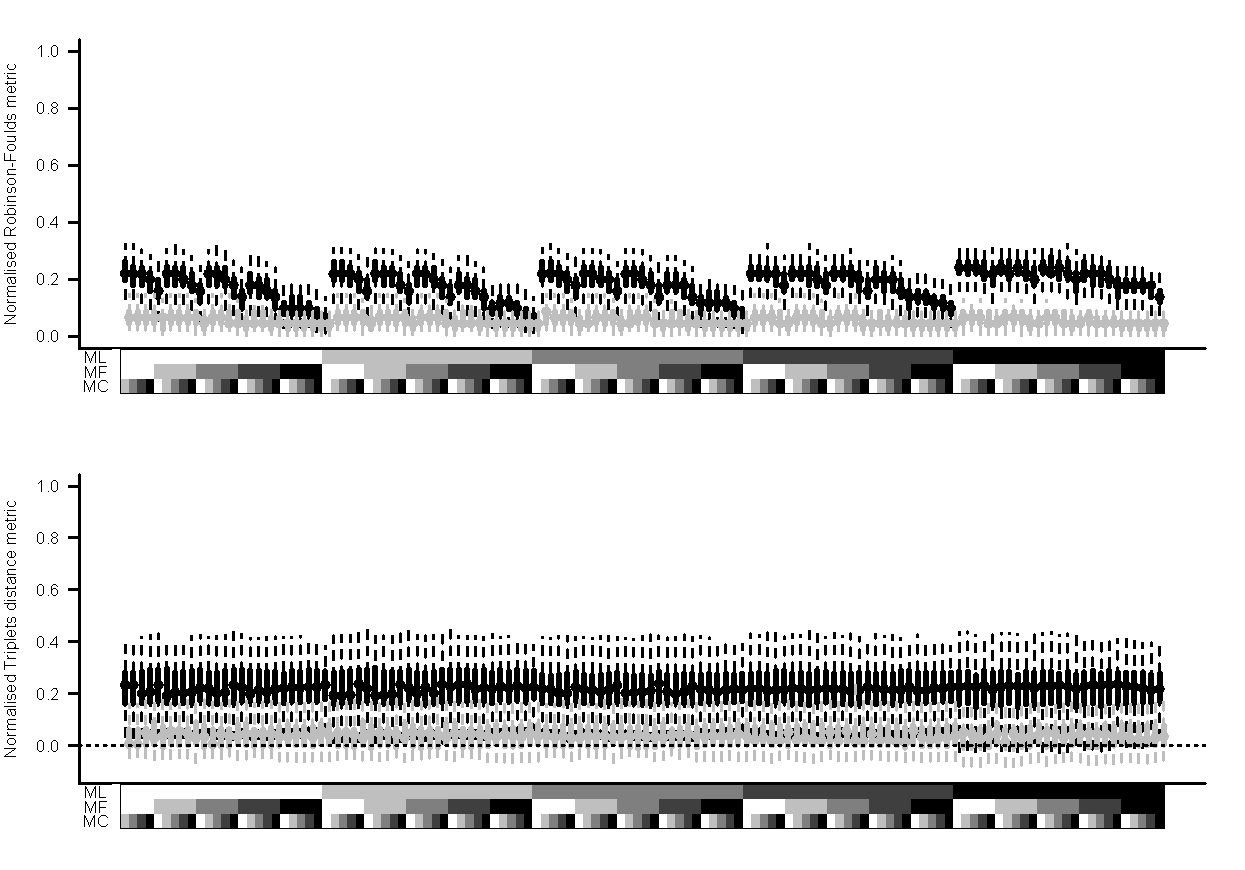
\includegraphics[width=1\textwidth]{SupplementaryFigures/Treesets_True.pdf}
    \caption{Effect of increasing missing data on topological recovering the ``true'' tree topology (the tree used for starting our simulations) for the Maximum Likelihood Bootstrap trees (black) and Bayesian posterior tree distribution (grey). The x axis shows the percentage of missing data from 0\% (white) to 75\% (black) for the two parameters: $M_{L}$ (upper line), $M_{F}$ (middle line) and number of characters from 100 to 25 for the parameter $N_{C}$ (lower line). Topological recovery was measured using two different tree comparison metrics: Normalised Robinson-Foulds metric (upper row) and Normalised Triplets metric (lower row). The graph shows the modal value (points), and the 50\% (thick solid lines) and 95\% (thin dashed lines) confidence intervals of the distributions of the tree comparison metric for each missing data parameter and tree inference method.} 
\label{Fig_Supp_Treesets_true} 
\end{figure}


%Summary of metrics values for all parameters combinations
\begin{landscape}
\begin{table}[ht]
\caption{Summary of the comparisons between the "best" tree and the "missing data" trees for each different tree inference method using either the Normalised Robinson-Foulds metric (RF) or the Normalised Triplets metric (Tr).}
\label{Tab_Supp_summary_metric_allparam}
\centering
\begin{tabular}{lccccccc}
  \hline
 Tree inference method & Metric & Min. & 1st Qu. & Median & Mean & 3rd Qu. & Max. \\ 
  \hline
  Maximum Likelihood                    & $RF$ & 0.06 & 0.26 & 0.40 & 0.41 & 0.50 & 0.95 \\ 
                                        & $Tr$ & 0.29 & 0.45 & 0.59 & 0.63 & 0.84 & 1.00 \\ 
  Bayesian consensus                    & $RF$ & 0.69 & 0.71 & 0.72 & 0.76 & 0.79 & 0.96 \\ 
                                        & $Tr$ & -0.28 & -0.11 & 0.17 & 0.19 & 0.37 & 0.98 \\ 
  Maximum Likelihood bootstraps         & $RF$ & 0.06 & 0.18 & 0.27 & 0.26 & 0.34 & 0.46 \\ 
                                        & $Tr$ & 0.23 & 0.31 & 0.35 & 0.38 & 0.45 & 0.58 \\ 
  Bayesian posterior tree distributions & $RF$ & 0.16 & 0.22 & 0.32 & 0.34 & 0.42 & 0.65 \\ 
                                        & $Tr$ & 0.24 & 0.35 & 0.40 & 0.50 & 0.67 & 0.98 \\ 
   \hline
\end{tabular}
\end{table}
\end{landscape}


%Summary of metrics values for the ML parameter
\begin{landscape}
\begin{table}[ht]
\caption{Summary of the comparisons between the "best" tree and the "missing data" trees for each different tree inference method using either the Normalised Robinson-Foulds metric (RF) or the Normalised Triplets metric (Tr) for the $M_{L}$ missing data parameter only.}
\label{Tab_Supp_summary_metric_ML}
\centering
\begin{tabular}{lccccccc}
  \hline
 Tree inference method & Metric & Min. & 1st Qu. & Median & Mean & 3rd Qu. & Max. \\ 
  \hline
  Maximum Likelihood                    & $RF$ & 0.44 & 0.51 & 0.63 & 0.66 & 0.78 & 0.95 \\ 
                                        & $Tr$ & 0.45 & 0.56 & 0.76 & 0.74 & 0.93 & 0.99 \\ 
  Bayesian consensus                    & $RF$ & 0.71 & 0.73 & 0.80 & 0.82 & 0.88 & 0.95 \\ 
                                        & $Tr$ & 0.37 & 0.46 & 0.67 & 0.67 & 0.87 & 0.96 \\ 
  Maximum Likelihood bootstraps         & $RF$ & 0.34 & 0.37 & 0.42 & 0.41 & 0.44 & 0.46 \\ 
                                        & $Tr$ & 0.32 & 0.40 & 0.51 & 0.46 & 0.51 & 0.57 \\ 
  Bayesian posterior tree distributions & $RF$ & 0.33 & 0.41 & 0.52 & 0.50 & 0.60 & 0.65 \\ 
                                        & $Tr$ & 0.41 & 0.56 & 0.76 & 0.71 & 0.84 & 0.98 \\ 
   \hline
\end{tabular}
\end{table}
\end{landscape}


%Summary of metrics values for the MF parameter
\begin{landscape}
\begin{table}[ht]
\caption{Summary of the comparisons between the "best" tree and the "missing data" trees for each different tree inference method using either the Normalised Robinson-Foulds metric (RF) or the Normalised Triplets metric (Tr) for the $M_{F}$ missing data parameter only.}
\label{Tab_Supp_summary_metric_MF}
\centering
\begin{tabular}{lccccccc}
  \hline
 Tree inference method & Metric & Min. & 1st Qu. & Median & Mean & 3rd Qu. & Max. \\ 
  \hline
  Maximum Likelihood                    & $RF$ & 0.23 & 0.46 & 0.64 & 0.61 & 0.79 & 0.93 \\ 
                                        & $Tr$ & 0.65 & 0.84 & 0.95 & 0.89 & 0.99 & 1.00 \\ 
  Bayesian consensus                    & $RF$ & 0.72 & 0.77 & 0.86 & 0.85 & 0.94 & 0.96 \\ 
                                        & $Tr$ & -0.16 & 0.19 & 0.63 & 0.52 & 0.96 & 0.98 \\ 
  Maximum Likelihood bootstraps         & $RF$ & 0.14 & 0.30 & 0.40 & 0.35 & 0.45 & 0.46 \\ 
                                        & $Tr$ & 0.37 & 0.49 & 0.54 & 0.51 & 0.56 & 0.57 \\ 
  Bayesian posterior tree distributions & $RF$ & 0.24 & 0.45 & 0.57 & 0.51 & 0.63 & 0.65 \\ 
                                        & $Tr$ & 0.44 & 0.81 & 0.86 & 0.82 & 0.98 & 0.98 \\ 
   \hline
\end{tabular}
\end{table}
\end{landscape}

%Summary of metrics values for the MC parameter
\begin{landscape}
\begin{table}[ht]
\caption{Summary of the comparisons between the "best" tree and the "missing data" trees for each different tree inference method using either the Normalised Robinson-Foulds metric (RF) or the Normalised Triplets metric (Tr) for the $N_{C}$ missing data parameter only.}
\label{Tab_Supp_summary_metric_MC}
\centering
\begin{tabular}{lccccccc}
  \hline
 Tree inference method & Metric & Min. & 1st Qu. & Median & Mean & 3rd Qu. & Max. \\ 
  \hline
  Maximum Likelihood                    & $RF$ & 0.40 & 0.50 & 0.64 & 0.65 & 0.79 & 0.94 \\ 
                                        & $Tr$ & 0.70 & 0.84 & 0.93 & 0.89 & 0.99 & 1.00 \\ 
  Bayesian consensus                    & $RF$ & 0.76 & 0.79 & 0.86 & 0.86 & 0.92 & 0.96 \\ 
                                        & $Tr$ & 0.05 & 0.16 & 0.53 & 0.50 & 0.87 & 0.92 \\ 
  Maximum Likelihood bootstraps         & $RF$ & 0.25 & 0.34 & 0.42 & 0.38 & 0.45 & 0.46 \\ 
                                        & $Tr$ & 0.38 & 0.47 & 0.55 & 0.51 & 0.57 & 0.58 \\ 
  Bayesian posterior tree distributions & $RF$ & 0.32 & 0.44 & 0.58 & 0.52 & 0.62 & 0.65 \\ 
                                        & $Tr$ & 0.39 & 0.78 & 0.82 & 0.79 & 0.98 & 0.98 \\ 
   \hline
\end{tabular}
\end{table}
\end{landscape}


%Summary of the BC between pairs of methods for the ML parameter
\begin{landscape}
\begin{table}[ht]
\caption{Bhattacharyya Coefficients of the pairwise method comparisons, each of which corresponds to the normalised metric between the "best" tree and the "missing data" using either the Normalised Robinson-Foulds metric (RF) or the Normalised Triplets metric (Tr) for the $M_{L}$ missing data parameter only.}
\label{Tab_Supp_summary_BC_ML}
\centering
\begin{tabular}{lccccccc}
  \hline
 Comparison &  Metric & Min. & 1st Qu. & Median & Mean & 3rd Qu. & Max. \\ 
  \hline
    Maximum Likelihood \textit{vs.} Bayesian consensus                 & $RF$ & 0.30 & 0.31 & 0.69 & 0.61 & 0.77 & \textbf{1.00} \\ 
                                                                       & $Tr$ & 0.79 & 0.81 & 0.84 & 0.86 & 0.85 & \textbf{1.00} \\ 
    Maximum Likelihood \textit{vs.} Maximum Likelihood bootstraps      & $RF$ & \textbf{0.03} & 0.22 & 0.29 & 0.36 & 0.54 & 0.69 \\ 
                                                                       & $Tr$ & 0.08 & 0.42 & 0.53 & 0.51 & 0.74 & 0.78 \\ 
    Maximum Likelihood \textit{vs.} Bayesian posterior trees           & $RF$ & \textbf{0.02} & 0.49 & 0.61 & 0.51 & 0.67 & 0.74 \\ 
                                                                       & $Tr$ & 0.21 & 0.61 & 0.70 & 0.63 & 0.81 & 0.81 \\ 
    Bayesian consensus \textit{vs.} Maximum Likelihood bootstraps      & $RF$ & \textbf{0.01} & \textbf{0.02} & \textbf{0.02} & \textbf{0.02} & \textbf{0.03} & \textbf{0.04} \\ 
                                                                       & $Tr$ & 0.08 & 0.69 & 0.78 & 0.64 & 0.79 & 0.84 \\ 
    Bayesian consensus \textit{vs.} Bayesian posterior trees           & $RF$ & \textbf{0.01} & \textbf{0.02} & \textbf{0.02} & \textbf{0.04} & 0.08 & 0.09 \\ 
                                                                       & $Tr$ & 0.21 & 0.74 & 0.75 & 0.68 & 0.84 & 0.87 \\ 
    Bayesian posterior tree \textit{vs.} Maximum Likelihood bootstraps & $RF$ & 0.69 & 0.75 & 0.85 & 0.85 & \textbf{0.95} & \textbf{1.00} \\ 
                                                                       & $Tr$ & 0.91 & 0.92 & \textbf{0.96} & \textbf{0.95} & \textbf{0.97} & \textbf{0.98} \\ 
   \hline
\end{tabular}
\end{table}
\end{landscape}

%Summary of the BC between pairs of methods for the MF parameter
\begin{landscape}
\begin{table}[ht]
\caption{Bhattacharyya Coefficients of the pairwise method comparisons, each of which corresponds to the normalised metric between the "best" tree and the "missing data" using either the Normalised Robinson-Foulds metric (RF) or the Normalised Triplets metric (Tr) for the $M_{F}$ missing data parameter only.}
\label{Tab_Supp_summary_BC_MF}
\centering
\begin{tabular}{lccccccc}
  \hline
 Comparison &  Metric & Min. & 1st Qu. & Median & Mean & 3rd Qu. & Max. \\  
  \hline
    Maximum Likelihood \textit{vs.} Bayesian consensus                 & $RF$ & \textbf{0.00} & 0.25 & 0.48 & 0.50 & 0.76 & \textbf{1.00} \\ 
                                                                       & $Tr$ & 0.38 & 0.69 & 0.75 & 0.72 & 0.80 & \textbf{1.00} \\ 
    Maximum Likelihood \textit{vs.} Maximum Likelihood bootstraps      & $RF$ & \textbf{0.03} & 0.18 & 0.32 & 0.36 & 0.47 & 0.77 \\ 
                                                                       & $Tr$ & 0.08 & 0.34 & 0.40 & 0.38 & 0.53 & 0.55 \\ 
    Maximum Likelihood \textit{vs.} Bayesian posterior trees           & $RF$ & \textbf{0.02} & 0.47 & 0.71 & 0.60 & 0.86 & 0.94 \\ 
                                                                       & $Tr$ & 0.21 & 0.54 & 0.62 & 0.56 & 0.64 & 0.80 \\ 
    Bayesian consensus \textit{vs.} Maximum Likelihood bootstraps      & $RF$ & \textbf{0.00} & \textbf{0.00} & \textbf{0.01} & \textbf{0.01} & \textbf{0.01} & \textbf{0.03} \\ 
                                                                       & $Tr$ & 0.08 & 0.38 & 0.54 & 0.49 & 0.70 & 0.75 \\ 
    Bayesian consensus \textit{vs.} Bayesian posterior trees           & $RF$ & \textbf{0.00} & \textbf{0.02} & \textbf{0.02} & \textbf{0.02} & \textbf{0.04} & \textbf{0.04} \\ 
                                                                       & $Tr$ & 0.21 & 0.29 & 0.66 & 0.54 & 0.72 & 0.82 \\ 
    Bayesian posterior tree \textit{vs.} Maximum Likelihood bootstraps & $RF$ & 0.69 & 0.69 & 0.72 & 0.71 & 0.72 & 0.72 \\ 
                                                                       & $Tr$ & 0.91 & 0.91 & 0.91 & 0.93 & 0.92 & \textbf{0.98} \\ 
   \hline
\end{tabular}
\end{table}
\end{landscape}

%Summary of the BC between pairs of methods for the MC parameter
\begin{landscape}
\begin{table}[ht]
\caption{Bhattacharyya Coefficients of the pairwise method comparisons, each of which corresponds to the normalised metric between the "best" tree and the "missing data" using either the Normalised Robinson-Foulds metric (RF) or the Normalised Triplets metric (Tr) for the $N_{C}$ missing data parameter only.}
\label{Tab_Supp_summary_BC_MC}
\centering
\begin{tabular}{lccccccc}
  \hline
 Comparison &  Metric & Min. & 1st Qu. & Median & Mean & 3rd Qu. & Max. \\  
  \hline
    Maximum Likelihood \textit{vs.} Bayesian consensus                 & $RF$ & \textbf{0.03} & 0.32 & 0.66 & 0.55 & 0.75 & \textbf{1.00} \\ 
                                                                       & $Tr$ & 0.51 & 0.69 & 0.80 & 0.76 & 0.80 & \textbf{1.00} \\ 
    Maximum Likelihood \textit{vs.} Maximum Likelihood bootstraps      & $RF$ & \textbf{0.03} & 0.17 & 0.21 & 0.31 & 0.46 & 0.68 \\ 
                                                                       & $Tr$ & 0.08 & 0.31 & 0.39 & 0.39 & 0.56 & 0.61 \\ 
    Maximum Likelihood \textit{vs.} Bayesian posterior trees           & $RF$ & \textbf{0.02} & 0.44 & 0.47 & 0.52 & 0.78 & 0.90 \\ 
                                                                       & $Tr$ & 0.21 & 0.52 & 0.59 & 0.55 & 0.66 & 0.77 \\ 
    Bayesian consensus \textit{vs.} Maximum Likelihood bootstraps      & $RF$ & \textbf{0.00} & \textbf{0.01} & \textbf{0.01} & \textbf{0.02} & \textbf{0.02} & \textbf{0.03} \\ 
                                                                       & $Tr$ & 0.08 & 0.47 & 0.62 & 0.51 & 0.66 & 0.73 \\ 
    Bayesian consensus \textit{vs.} Bayesian posterior trees           & $RF$ & \textbf{0.00} & \textbf{0.02} & \textbf{0.04} & \textbf{0.04} & 0.05 & 0.06 \\ 
                                                                       & $Tr$ & 0.21 & 0.45 & 0.64 & 0.57 & 0.74 & 0.79 \\ 
    Bayesian posterior tree \textit{vs.} Maximum Likelihood bootstraps & $RF$ & 0.69 & 0.73 & 0.73 & 0.76 & 0.81 & 0.86 \\ 
                                                                       & $Tr$ & 0.91 & 0.92 & 0.93 & 0.94 & \textbf{0.96} & \textbf{0.99} \\ 
   \hline
\end{tabular}
\end{table}
\end{landscape}

\begin{table}[ht]
\caption{Summary of the median Bhattacharyya Coefficients comparisons between the missing data parameters. Each value corresponds to the median Bhattacharyya Coefficient between the Normalised metrics (Robinson-Foulds - RF; Triplets - Tr) between the ``best'' and the ``missing data'' trees (as outlined in Figure 2 in the main text) for the the trees with: Missing Living taxa only ($M_L$); Missing Fossil data only ($M_F$); Number of characters only ($N_C$); and the combination of the three parameters (combined).} 
\begin{tabular}{llcccc}  
  \hline
 Method & Metric & $M_L$ & $M_F$ & $N_C$ & combined \\ 
  \hline
Maximum Likelihood & RF & 0.54 & 0.37 & 0.56 & 0.54 \\ 
                   & Tr & 0.80 & 0.75 & 0.80 & 0.79 \\ 
Bayesian consensus & RF & 0.73 & 0.59 & 0.60 & 0.79 \\ 
                   & Tr & 0.86 & 0.67 & 0.81 & 0.81 \\ 
Maximum Likelihood bootstraps & RF & \textbf{0.98} & \textbf{0.96} & \textbf{0.97} & 0.78 \\ 
                   & Tr & \textbf{0.99} & \textbf{1.00} & \textbf{1.00} & \textbf{0.96} \\ 
Bayesian posterior trees & RF & 0.86 & 0.93 & 0.94 & 0.68 \\ 
                   & Tr & \textbf{0.98} & \textbf{0.99} & \textbf{0.99} & 0.91 \\ 
 \hline
\end{tabular}
\end{table}

\begin{table}[ht]
\caption{Summary of the median Bhattacharyya Coefficients comparisons between the missing data parameters and the methods. Each value corresponds to the median Bhattacharyya Coefficient between the Normalised metrics (Robinson-Foulds - RF; Triplets - Tr) between the `methods (as outlined in Figure 3 in the main text) for the the trees with: Missing Living taxa only ($M_L$); Missing Fossil data only ($M_F$); Number of characters only ($N_C$); and the combination of the three parameters (combined).}
\begin{tabular}{llcccc}  
  \hline
 Method & Metric & $M_L$ & $M_F$ & $N_C$ & combined \\ 
  \hline
Maximum likelihood vs. Bayesian consensus & RF & 0.69 & 0.48 & 0.66 & 0.10 \\ 
   & Tr & 0.84 & 0.75 & 0.80 & 0.61 \\ 
Maximum likelihood vs. Bootstraps & RF & 0.29 & 0.32 & 0.21 & 0.69 \\ 
   & Tr & 0.53 & 0.40 & 0.39 & 0.65 \\ 
Maximum likelihood vs. Bayesian posterior trees & RF & 0.61 & 0.71 & 0.47 & 0.80 \\ 
  & Tr & 0.70 & 0.62 & 0.59 & 0.73 \\ 
Bayesian consensus vs. Bootstraps & RF & \textbf{0.02} & \textbf{0.01} & \textbf{0.01} & \textbf{0.00} \\ 
  & Tr & 0.78 & 0.54 & 0.62 & 0.59 \\ 
Bayesian consensus vs. Bayesian posterior trees & RF & \textbf{0.02} & \textbf{0.02} & \textbf{0.04} & \textbf{0.01} \\ 
   & Tr & 0.75 & 0.66 & 0.64 & 0.56 \\ 
Boostraps vs. Bayesian posterior trees & RF & 0.85 & 0.72 & 0.73 & 0.85 \\ 
   & Tr & \textbf{0.96} & 0.91 & 0.93 & \textbf{0.98} \\ 
 \hline
\end{tabular}
\end{table}
%END
\end{document}